\documentclass[12pt]{iopart} % Document class declaration

% package "imports"
\usepackage{graphicx}
\usepackage{IEEEtrantools}

% Custom macros
\gdef\mcm{r@{.}l@{ ± }r@{.}l} % Multi Column Measurement; Used for decimal aligning & ± aligning
\gdef\mch#1{\multicolumn{4}{l}{#1}} % Multi Column Header; Used for decimal aligning & ± aligning
\gdef\mcmnd{r@{ ± }l} % Multi Column Measurement No Decimal; Used for ± aligning when the values don't need a decimal point
\gdef\mchnd#1{\multicolumn{2}{l}{#1}} % Multi Column Header No Decimal; Used for  ± aligning when the values don't need a decimal point
\gdef\sci#1#2{#1 \times 10^{#2}}
\gdef\units#1{~\mathrm{#1}}

%%%%%%%%%%%%%%%%%%%% Document Starts %%%%%%%%%%%%%%%%%%%%
\begin{document}

%%%%%%%%%%%%%%%%%%%% Title Page %%%%%%%%%%%%%%%%%%%%
\title{Realistic Projectiles}
\author{Ali Mortada, Xavier Valencia, James Phommachanh, Wes Cochran}
\vspace{10pt}
\begin{indented}
  \item[]Mt.~San Antonio College, ENGR 285, CRN 43464
  \item[]May 20, 2024
\end{indented}
\newpage

%%%%%%%%%%%%%%%%%%%% Objectives %%%%%%%%%%%%%%%%%%%%
\section{Objectives}

\begin{center}
\subtitle{\textbf{Interdependence of Motion}}
\end{center}

Blah blah blah.

% how to do el figure
%\begin{figure}[h!tbp]
%  \begin{center}
% \item[]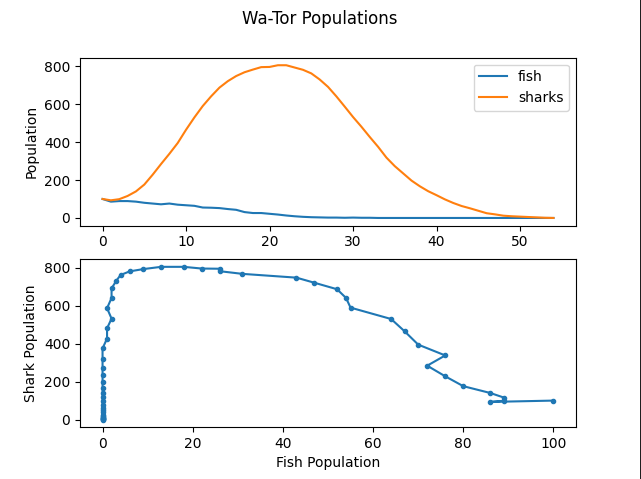
\includegraphics[width=0.6\textwidth]{figure1.png}
%  \caption{\label{fig:figure1}
%  Outcome one when \emph{energy\_gain} has the highest step with a random distribution.
%  }
%  \end{center}
%\end{figure}


\pagebreak

\begin{center}
\subtitle{\textbf{Trajectories}}
\end{center}

Blah blah blah 2.

\pagebreak

\begin{center}
\subtitle{\textbf{Firing Range}}
\end{center}

Blah blah blah 3.


\pagebreak

%%%%%%%%%%%%%%%%%%%% Extension %%%%%%%%%%%%%%%%%%%%
\section{Extension: Incorporating Lift}

Do you even lift bro?

\end{document}
%%%%%%%%%%%%%%%%%%%% Document Ends %%%%%%%%%%%%%%%%%%%%